\section{Características del conjunto de datos} \label{specs}

      Se debe tener cuenta que el archivo de evento para todos los disparos no es comparable con el conjunto  de datos del ICRC 2019. Porque el primero es entre los años 2013 y 2019 y el segundo se adquieren usando el disparo estándar.  Algo a considerar es que la colaboración cambió el algoritmo de reconstrucción de eventos en el 2019, con respecto al 2017.

    %COMPARANDO DELTA E ENTRE LOS DOS ARCHIVOS
      En las  Figs.\,\ref{fig:deltaE} y \ref{fig:histograma} se muestra la diferencia entre el valor de energía entre eventos coincidentes entre las reconstrucciones del año 2017 y 2020. Puede apreciarse que la diferencia no esta centrada 0 y no aparenta tener una modulación del clima. Por lo tanto la diferencia se debe a una reconstrucción distinta de los eventos.

    %COMPARANDO LA CURVA DE CALIBRACIÓN ENTRE LOS DOS ARCHIVOS
      Puede verse en la Fig.\,\ref{fig:calibracionE} que la curva de calibración entre ambos archivos es distinta, ya que la coordenada al origen como la pendiente es difieren entre para ambos archivos. Esto implica que los valores A y B de la curva $E=A\times (S_{38})^B$ son distintos para ambos conjunto de datos. Esto afectaría en primer lugar en el valor de la energía, y segundo a cualquier análisis que dependan de estos parámetros, como el análisis de la modulación del clima.

	Además de los filtros aplicados mencionados en la sección \ref{filtro}, se aplican filtros adicionales sobre la energía y el rango de tiempo. Para estudiar los eventos en esta sección, consideramos los eventos entre 1\,EeV y 2\,EeV de energía y que ocurrieron entre las 12:00:00 GMT del 1 de enero de 2014 y las 12:00:00 GMT del 1 de enero de 2020. Se centró en este rango de tiempo, ya que el registro de eventos más reciente al que se tuvo para hacer este trabajo termina el 1 de Enero del 2020  a las 11:59:43 GMT, además de para estudiar una cantidad entera de años, se optó por considerar los eventos desde el 1 de Enero del 2014 a las 12:00:00 GMT.

	Un resumen de todos los filtros aplicados se encuentra a continuación
		\begin{enumerate}
			\item Son eventos obtenidos mediante todos los disparos.
			\item Energía entre  [1 EeV , 2 EeV)
			\item Rango de tiempo:
			\begin{itemize}
				\item[-] Inicial:Jueves, 1 de Enero de 2014 12:00:00 GMT o 1388577600 UTC
				\item[-] Final:  Jueves, 1 de Enero de 2020 12:00:00 GMT o 1577880000 UTC
			\end{itemize}

		\end{enumerate}
	Aplicando estos filtros, se tienen $1\,081\,844$ eventos para estudiar en este rango de energía. 


        \begin{figure}[H]
          \centering
            \begin{subfigure}[b]{0.65\textwidth}
              \centering
              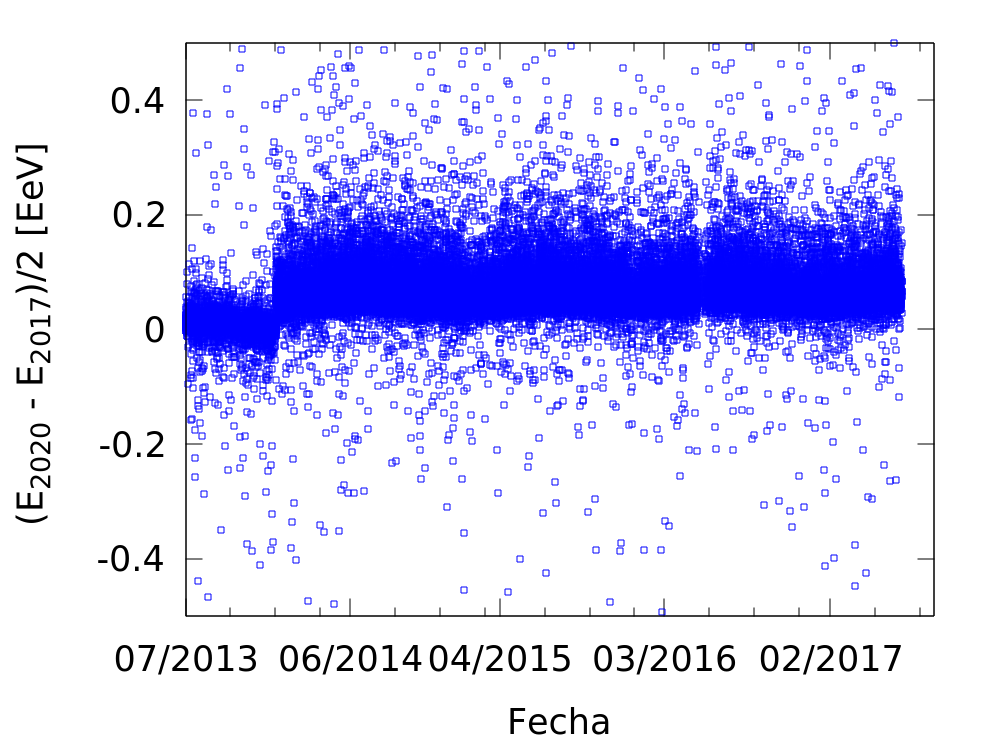
\includegraphics[width=\linewidth]{../0_Introduccion/comparacion_deltaE.png}
              \caption{Diferencia entre las energías} \label{fig:deltaE}
            \end{subfigure}\\
            \begin{subfigure}[b]{0.65\textwidth}
              \centering
              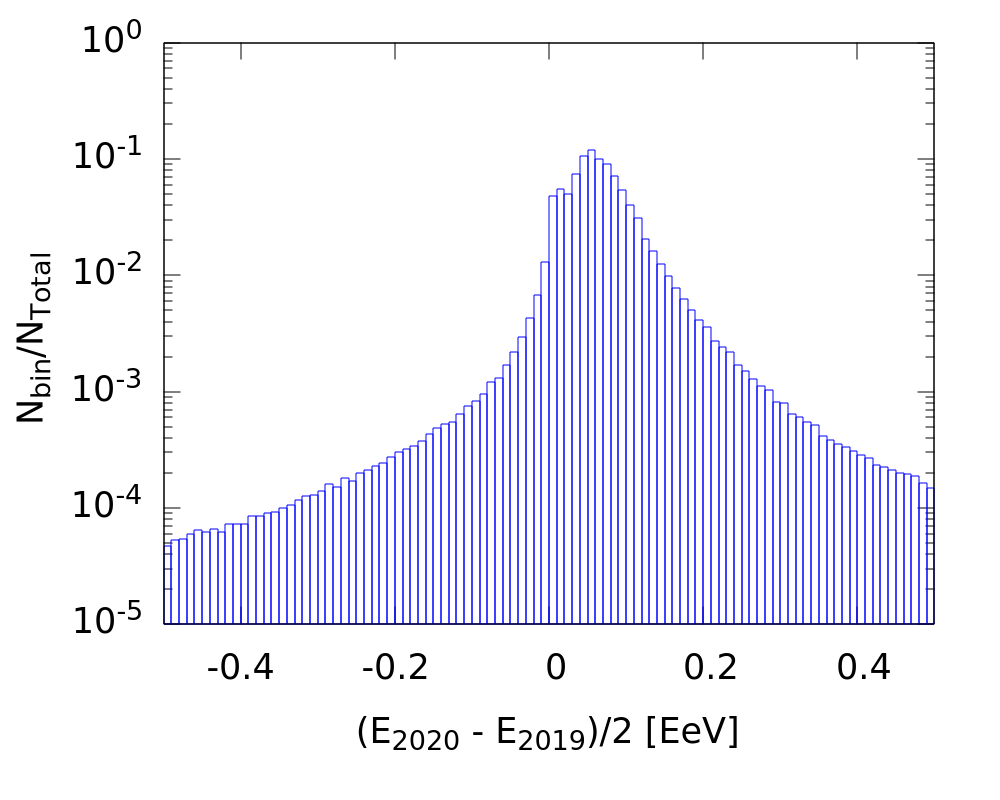
\includegraphics[width=\linewidth]{../0_Introduccion/histograma_deltaE.png}
              \caption{Histograma de las diferencias}   \label{fig:histograma}
            \end{subfigure}
           \caption{Diferencia entre las energías de entre la reconstrucción del 2017 y del 2019}
         \end{figure}

        \begin{figure}[H]
          \centering
          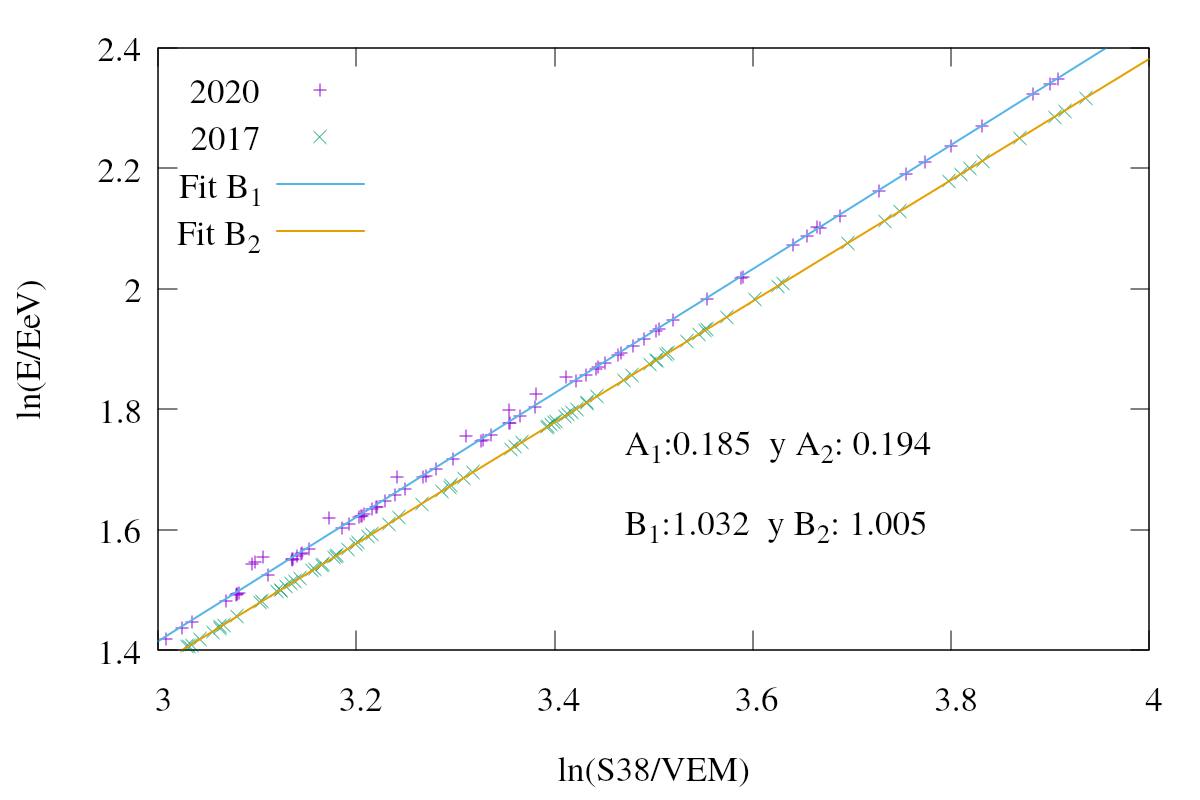
\includegraphics[width=0.65\textwidth]{../0_Introduccion/comparacion_reconstruccion.png}
          \caption{Calibración de las energías del archivo de 2017 y el archivo del 2019}
          \label{fig:calibracionE}
        \end{figure}
	
\section{Pesos de los eventos para frecuencias de referencia}

	 En la Fig.\,\ref{pesos_bin_1_2} se muestran los valores de  $\Delta N_{cell,k}$ en el rango donde se consideran los eventos. 
			 
			\begin{figure}[H]
				\centering
				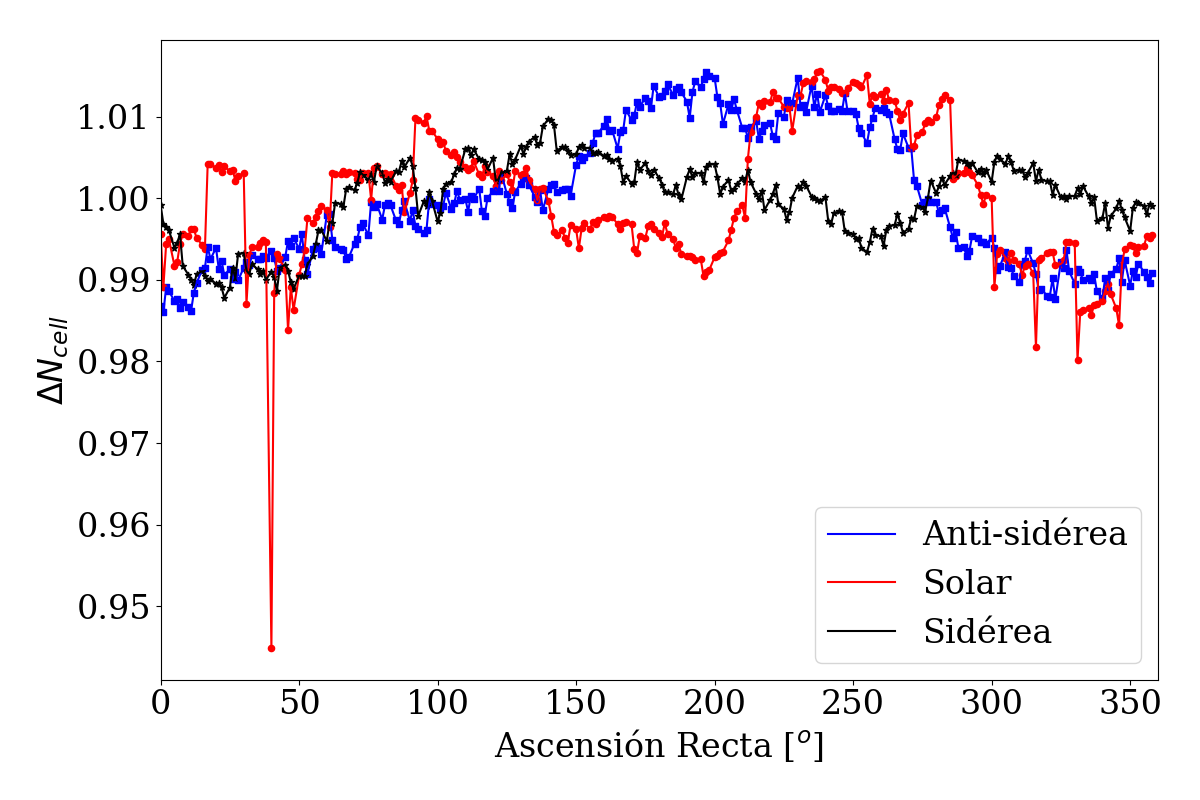
\includegraphics[width=0.75\textwidth]{weights_2013_2020.png}
				\caption{Variaciones de los hexágonos para frecuencias características en rango mencionado. }
				\label{pesos_bin_1_2}
			\end{figure}


	A cada una de estas frecuencias, se ajusta una función del tipo  $f(x)=a\cdot \cos{(\alpha-\phi)} + 1$, con el se busca aproximar la amplitud $a$ y el desfase $\phi$ de las curvas de los pesos en función de la ascensión recta $\alpha$. Los ajustes se observan en las Figs. \ref{fig:ajuste_antisiderea}, \ref{fig:ajuste_solar} y \ref{fig:ajuste_siderea}.


	\subsection{Gráficos de los ajustes}

Para verificar los valores de amplitud y fase en la frecuencia sidérea, se ajusta una función del tipo 
\begin{equation}
	f(RA) = a\cos{(2\pi(\omega RA + \phi))} +c
\end{equation}

a la variación de los hexágonos por ángulos de ascensión recta $RA$, así como también a la variación de los pesos de los eventos en ascensión recta \footnote{El peso de los eventos es la inversa del peso de los hexágonos}. En el ajuste, se dejan libres los parámetros de la amplitud $a$, desfase $\phi$ y offset $c$, en cambio la frecuencia $\omega=1$, ya que los valores de ascensión recta $0^o$ y $360^o$ son equivalentes y estamos trabajando con el primer armónico. La variación y el ajuste puede verse en las Figs.%\ref{fig:pesos_ajuste} y \ref{fig:pesos_hexagonos}.

Los valores de los ajustes, comparados con el análisis de Rayleigh se muestran en la Tabla\,\ref{tabla:ajuste_primer_armonico}. SE observa que el valor de la amplitud para el caso de la variación de los pesos es más cercana al que se obtuvo en el análisis de Rayleigh. Esto puede deberse que los pesos están normalizados por la integral de todos los hexágonos dada un frecuencia, por lo que si existe alguna constante multiplicativa en la cantidad de hexágonos, la amplitud la tabla para la primera columna puede no ser igual a la segunda columna.

\begin{table}[H]
\centering
\begin{tabular}{l|c|c|||c}
				& Hexágonos 				& Pesos	de los eventos		& Rayleigh con peso \\ \hline
%Figura:			& \ref{fig:pesos_hexagonos} &\ref{fig:pesos_ajuste}		&\ref{fig:zoom} \\
Fase $\phi$:	& 284.874 	 				& 285.099					&329.865	\\
Amplitud $a$:	& 0.00784107 				&  0.00384774 				&0.004676\\
\end{tabular}
\caption{Fase y amplitud del ajuste del primer armónico en ascensión recta en los hexágonos y  pesos  de los eventos para la frecuencia sidérea}
\label{tabla:ajuste_primer_armonico}
\end{table}


		
		\begin{figure}[H]
		\centering
		\begin{subfigure}{.75\textwidth}
			\centering
			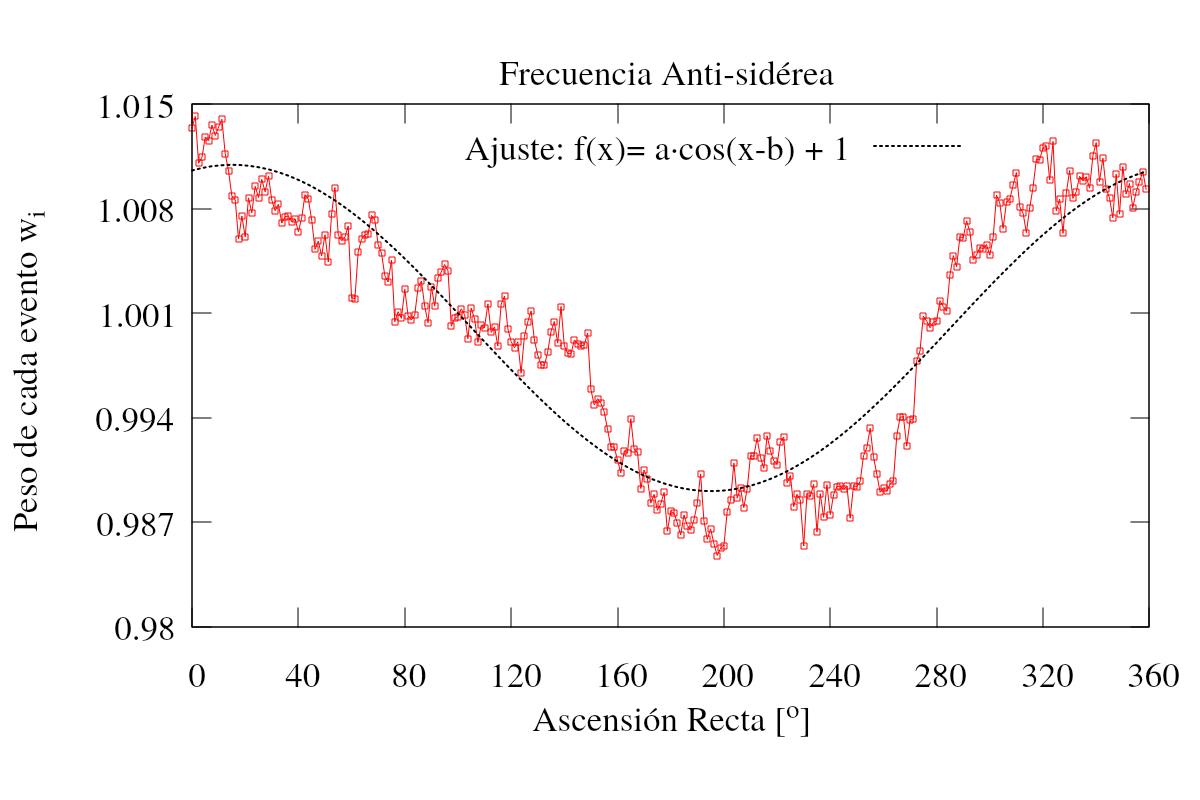
\includegraphics[width=\linewidth]{eventos_RA_ajuste_cos_antisiderea_v2.png}
			\caption{Frecuencia anti-sidérea}
			\label{fig:ajuste_antisiderea}
		\end{subfigure}\\
		\begin{subfigure}{.75\textwidth}
			\centering
			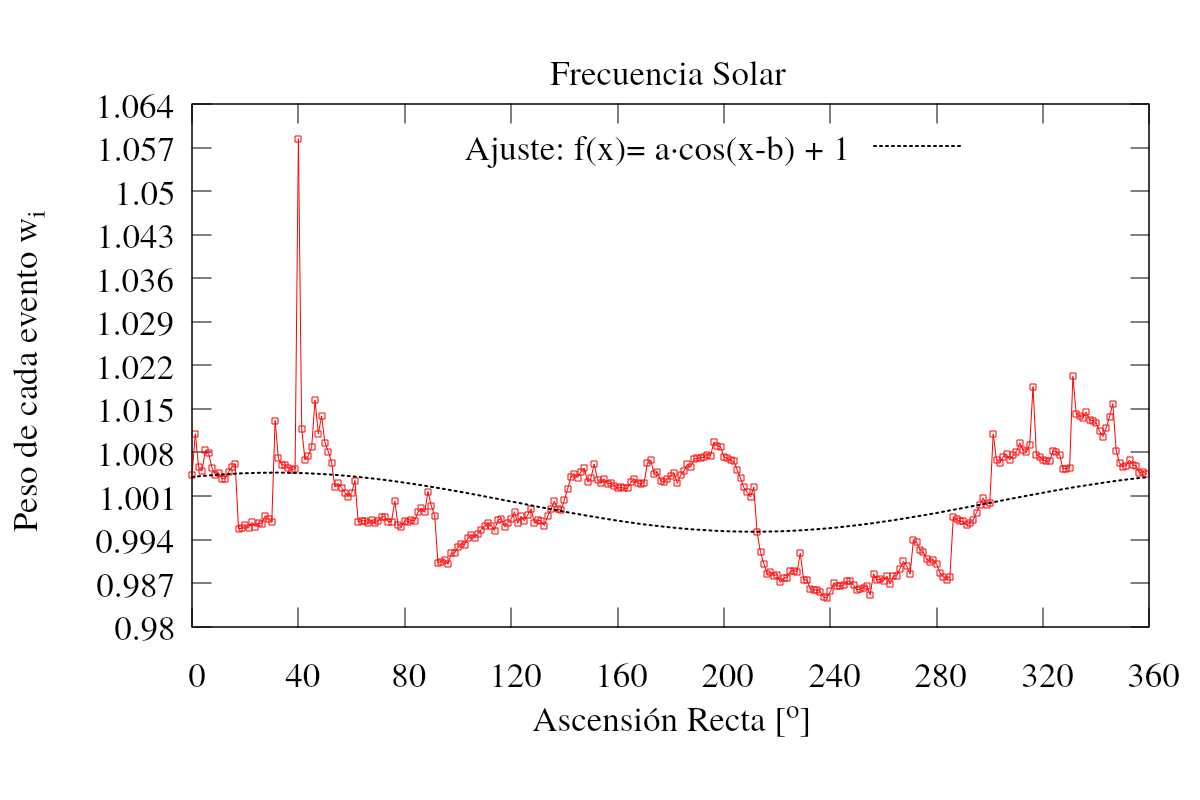
\includegraphics[width=\linewidth]{eventos_RA_ajuste_cos_solar_v3.png}
			\caption{Frecuencia solar}
			\label{fig:ajuste_solar}
		\end{subfigure}\\
		\centering
		\begin{subfigure}{.75\textwidth}
			\centering
			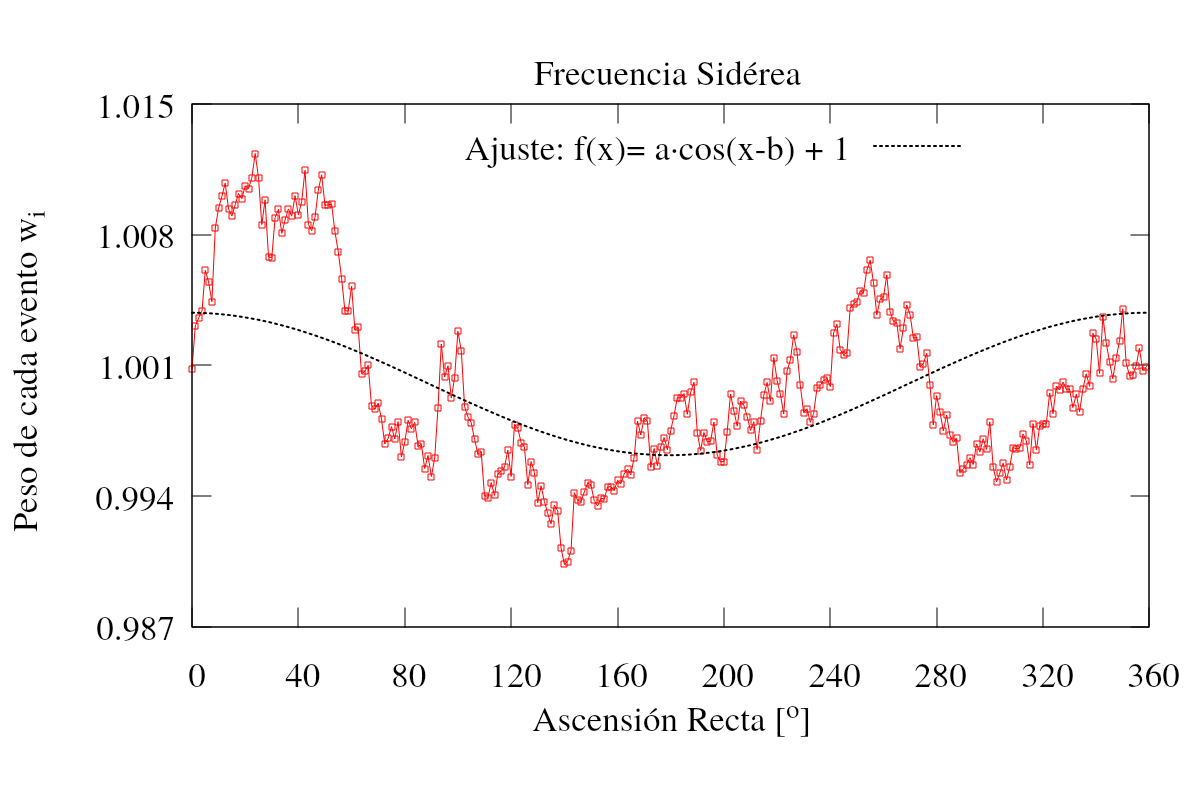
\includegraphics[width=\linewidth]{eventos_RA_ajuste_cos_siderea_v2.png}
			\caption{Frecuencia sidérea}
			\label{fig:ajuste_siderea}
		\end{subfigure}%
		\caption{Ajuste de los pesos de los eventos para varias frecuencias a primer orden en ascensión recta}
		\end{figure}
		
	
\subsection{Tabla comparando los ajustes:}
		
		\begin{table}[H]
		\centering
		\begin{tabular}{c|c|c|c}
					& Anti-sidérea			& Solar 				& Sidérea\\ \hline
		Amplitud $a$& $0.0109\pm 0.0003 $ 	&	$0.0038 \pm 0.0003$	&  $0.0047\pm 0.0007$		\\
		Fase $\phi$ & $15    \pm 1$ 		&   $360 \pm 5   $ 		&  $31    \pm 8    $ 		\\
		\end{tabular}
		\caption{Parámetros obtenidos del ajuste a primer orden en $\alpha$ sobre los pesos.}
		\end{table}


\section{Gráfico de la anisotropía}

 En las figuras de esta sección se muestran el análisis en ascensión recta para los eventos de observatorio considerando las variaciones de la exposición.

 Los mismos se hicieron en el mismo intervalo de tiempo para poder compararlos entre sí. 
 
%Elegí el rango presentado en la Tabla \ref{rango_corto}  porque en el mismo se encuentran todos los eventos filtrados por energía, por bad period, por reconstrucción correcta, etc.



% \begin{table}[H]
% \centering
% \begin{tabular}{l|c|c}
% 				& Con Peso 	& Sin peso 		\\ \hline
% Frecuencia:		& 366.25 	& 366.25 		\\
% Fase:			& 329.865 	& 292.312		\\
% $P(r)$:			& 0.76398\%	& 26.6838 \% 	\\
% Amplitud:		& 0.004676 	& 0.00243515	\\
% \end{tabular}
% \caption{Fase, $r_{99}$ y $P_{99}$ del análisis de anisotropía }
% \end{table}



%En la Fig.\ref{fig:zoom} se muestra el pico que se presenta en  el intervalo de energía entre 1 EeV - 2 EeV, cercano a la frecuencia sidérea. El pico tiene un máximo para un período de $366.21$. En la Tabla.\,\ref{tabla:pico} se muestran los valores de la fase, $r_{99}$ y $P_{99}$ para el periodo anterior.

% \begin{figure}[H]

	\subsubsection{Análisis de anisotropías en ascensión recta}
		
		\begin{figure}[H]
			\centering
			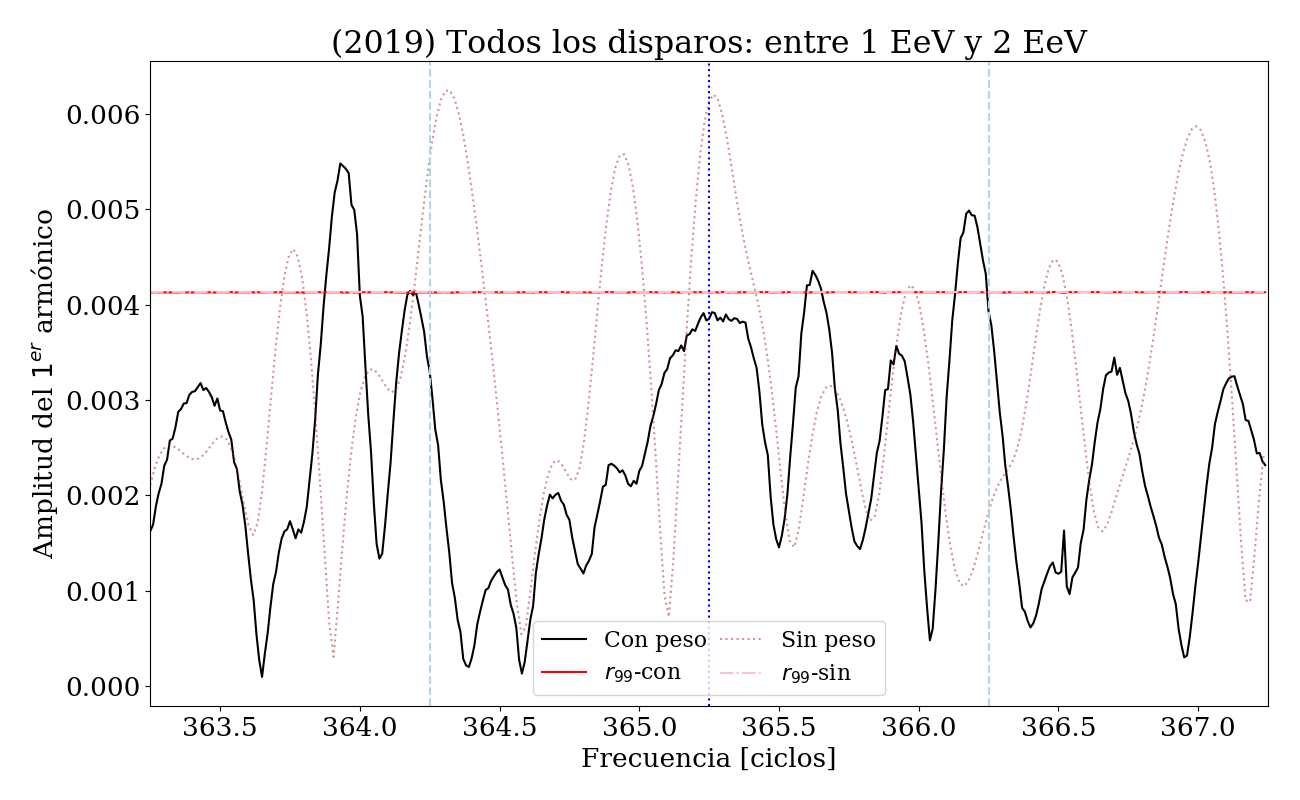
\includegraphics[width=0.75\linewidth]{pesos_sin_con_1_2_EeV.png}
			\caption{Anisotropía en función de la frecuencia, se comparan los análisis sin los pesos y con los pesos de los hexágonos}
		\end{figure}
		

		\begin{table}[H]
		\centering
		\begin{tabular}{l|l|l|l|l}
			\multicolumn{1}{c}{}  & \multicolumn{2}{c}{Sin pesos}  & \multicolumn{2}{|c}{Con pesos} \\ \hline
			Frecuencia:   & Solar         & Sidérea        & Solar         & Sidérea        \\ \hline
			Fase $\phi$:  & 251           & 289            & 288           & 335            \\ \hline
			Amplitud $r$: & 0.0061        & 0.0018         & 0.0038        & 0.0039         \\ \hline
			$P(r)$:	      & 0.004 \%	  & 41\%	   	   & 2 \%          & 1 \% 	\\
		\end{tabular}
		\caption{Comparación de los parámetros de fase y amplitud para las frecuencias sidérea y solar, analizando sin pesos y con los pesos de los hexágonos con el análisis de Rayleigh entre en 1 de Enero del 2014 y el 1 de Enero del 2020}
		\end{table}
		
		% \begin{table}[H]
		% \centering
		% \begin{tabular}{c|c|c|c|c|c}
		% Frecuencia	& Solar (sin peso)	& Solar (con peso)	&& Sidérea (sin peso) 	& Sidérea (con peso)	 \\ \hline
		% Fase $\phi$ & 251	    		& 288	    		&& 289				& 335				\\
		% Amplitud $r$& 0.0061	    	& 0.0038	  		&&0.0018		& 0.0039			\\
		% \end{tabular}

		% \end{table}

	\subsubsection{Bineado de eventos }


	Considerando que estamos trabajando con la frecuencia solar al hacer el análisis con pesos, se obtiene la siguiente distribución de eventos en función de su ascensión recta.
	\begin{figure}[H]
		\centering
		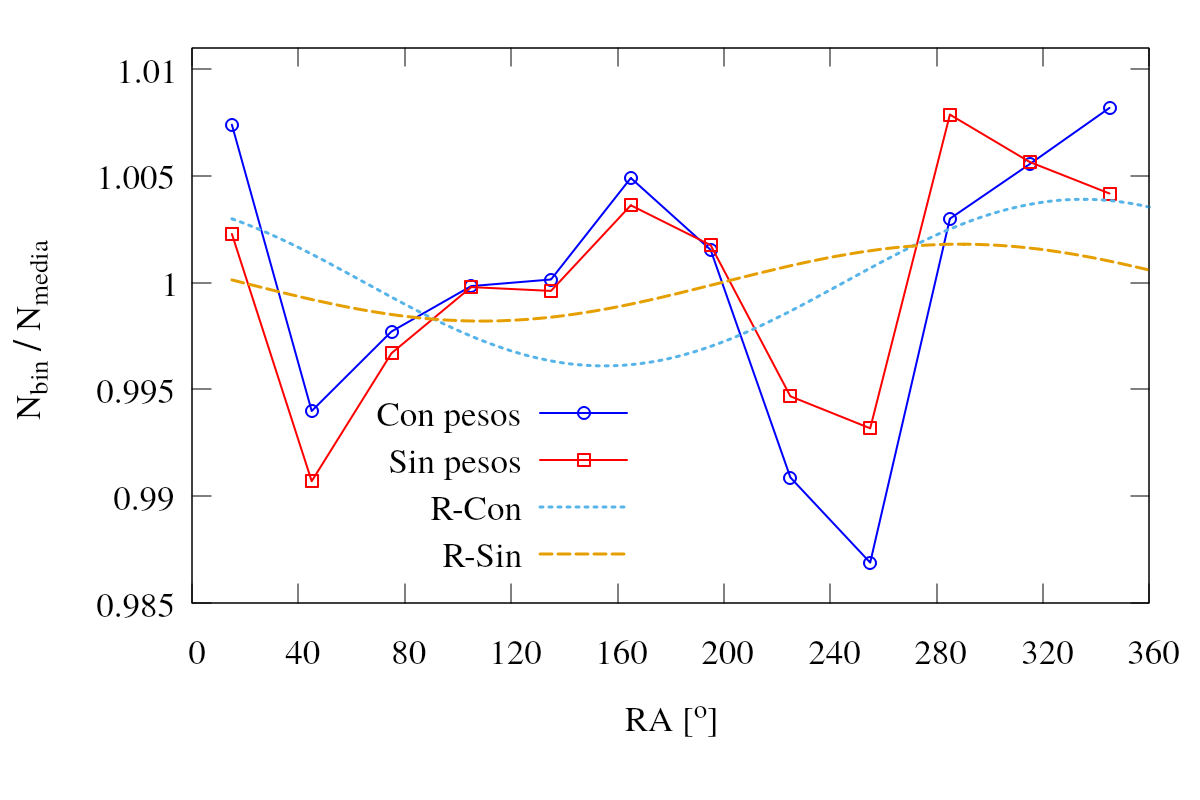
\includegraphics[width=0.75\linewidth]{eventos_clasificados_por_RA_v4.png}
		\caption{Distribución de la cantidad relativa de eventos en función de la ascensión recta a primer orden.}
	\end{figure}

	\begin{figure}[H]
		\centering
		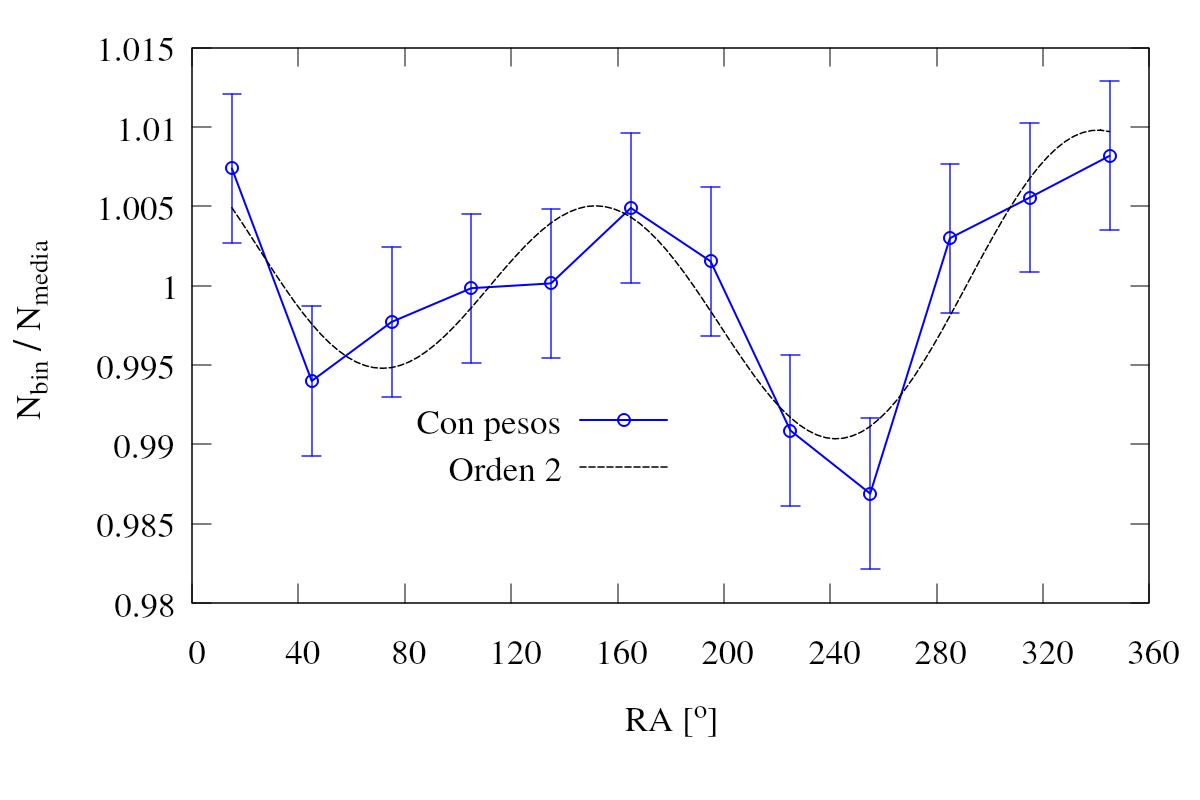
\includegraphics[width=0.75\linewidth]{eventos_clasificados_por_RA_v6_orden_2.png}
		\caption{Distribución de la cantidad relativa de eventos en función de la ascensión recta a segundo orden.}
	\end{figure}


La Figura 5.15 muestra la tasa de eventos normalizada en este intervalo de energía.
La línea continua es el valor del primer armónico obtenido a través del análisis de
Fourier. Es evidente que la modulación tiene características adicionales a las del primer
armónico, de hecho, el siguiente modo en valor de la amplitud es el cuarto, para el cual
$r 4 \alpha = 4.9 \times 10 -3 $con una probabilidad $P (>= r 4 \alpha ) = 2.7 \times 10 -3$ . La línea discontinua
muestra la distribución proveniente de la suma de los cuatro primeros armónicos. Es
interesante que el mayor exceso con respecto al caso dipolar es un salto en el intervalo
de ascensión recta $[ 270 ^o , 300 ^o ]$, muy cerca a la dirección del centro galáctico. Estudios
futuros de esta característica podrían ser interesantes para determinar su origen.

%%%%%%%%%%%%%%%%%%%%%%%%%5555

%%%%%%%%%%%%%%%%%%%%%%%%5

%%%%%%%%%%%%%%%%%%%%%%%%



% \begin{table}[H]
% \centering
% \begin{tabular}{l|c|c|c|c}
% 				& Con Peso 		& Sin peso 		& Con Peso 		& Sin peso 		\\ \hline
% Frecuencia:		& 366.21 		& 366.21 		& $\sim$366.505 & 366.506 		\\
% Fase:			& 151.032 		& 121.695		& $\sim$190 	& 73.8188		\\
% $P(r)$:		   & 0.289882\%	  & 46.9691 \% 	& $\sim$96\%	& 0.24013 \% 	\\
% Amplitud:		& 0.00512146	& 0.0018417		& $\sim$0.0006	& 0.00520328	\\
% \end{tabular}
% \caption{Fase, $r_{99}$ y $P_{99}$ del análisis de anisotropía entre en 1 de Enero del 2014 y el 1 de Enero del 2020}
% \label{tabla:pico}
% \end{table}


